\documentclass[12pt]{article}
\usepackage{amsmath, amssymb, amsthm}
\usepackage{graphicx}
\usepackage{geometry}
\usepackage{hyperref}

\geometry{a4paper, margin=1in}

\title{Kernel Canonical Correlation Analysis in Hilbert and \( L^2[a,b] \) Spaces}
\author{Bair Mikhailov}
\date{\today}

\begin{document}

\maketitle

\begin{abstract}
Kernel Canonical Correlation Analysis (Kernel CCA) is a powerful technique that extends the classical CCA by leveraging the kernel trick to capture nonlinear relationships between two sets of variables. In this article, we explore the foundations of Kernel CCA, its formulation in Hilbert spaces, and its specific application in \( L^2[a,b] \) spaces, which are important in functional data analysis.
\end{abstract}

\section{Introduction}

Canonical Correlation Analysis (CCA) is a classical multivariate statistical method that identifies linear relationships between two sets of variables. Given two random variables \( X \) and \( Y \), CCA seeks to find linear projections \( w_X^\top X \) and \( w_Y^\top Y \) such that the correlation between these projections is maximized. However, CCA is limited to linear relationships.

Kernel Canonical Correlation Analysis (Kernel CCA) extends CCA by mapping the data into a high-dimensional (or even infinite-dimensional) feature space through a nonlinear mapping, allowing it to capture complex relationships. This is particularly useful in machine learning and data analysis where the relationships between variables are often nonlinear.

\section{Kernel CCA in Hilbert Spaces}

Let \( \mathcal{H}_X \) and \( \mathcal{H}_Y \) be reproducing kernel Hilbert spaces (RKHS) associated with the random variables \( X \) and \( Y \) respectively, with kernels \( k_X(x, x') \) and \( k_Y(y, y') \). The key idea in Kernel CCA is to find functions \( f \in \mathcal{H}_X \) and \( g \in \mathcal{H}_Y \) such that the correlation between \( f(X) \) and \( g(Y) \) is maximized.

Mathematically, we seek to solve the following optimization problem:
\[
\max_{f \in \mathcal{H}_X, g \in \mathcal{H}_Y} \text{Corr}(f(X), g(Y)),
\]
subject to the norm constraints \( \|f\|_{\mathcal{H}_X} = 1 \) and \( \|g\|_{\mathcal{H}_Y} = 1 \).

This can be reformulated using the kernel trick, where the solutions \( f \) and \( g \) are expressed as linear combinations of the kernel functions:
\[
f(x) = \sum_{i=1}^n \alpha_i k_X(x_i, x), \quad g(y) = \sum_{j=1}^m \beta_j k_Y(y_j, y).
\]
The problem then reduces to finding the coefficients \( \alpha \) and \( \beta \) that maximize the correlation between these functions.

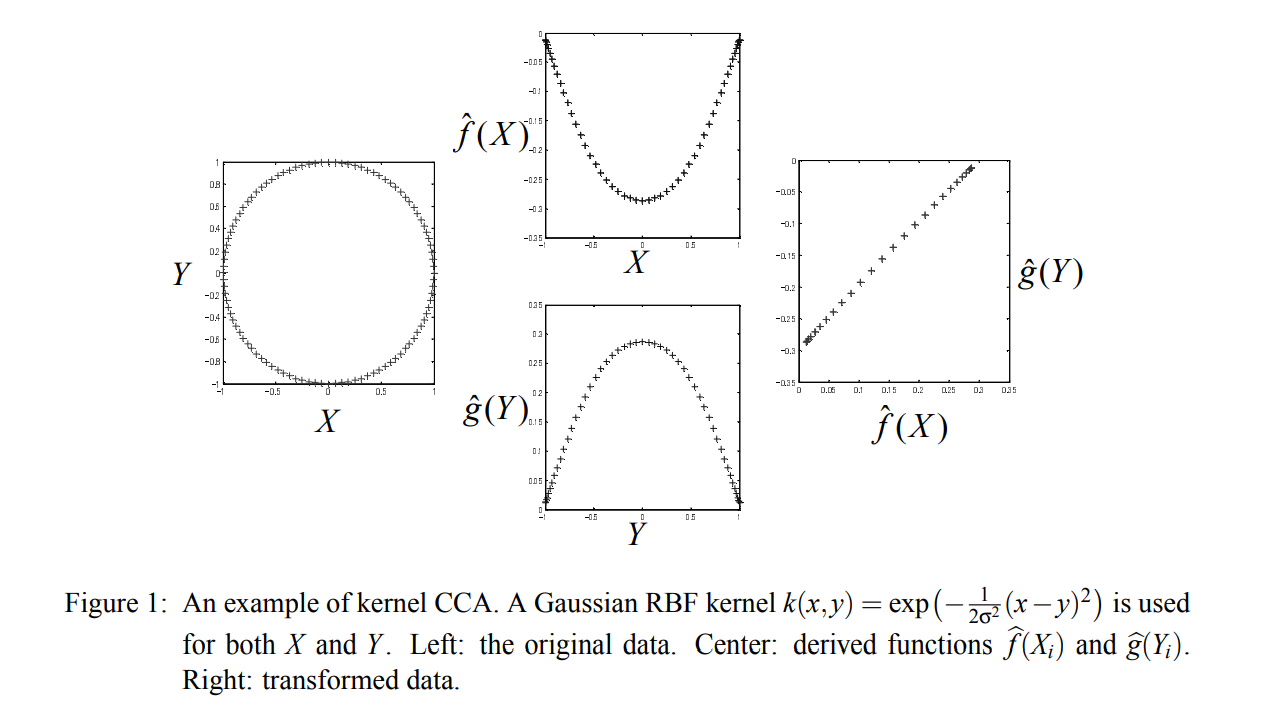
\includegraphics[scale=0.35]{tmp_example.png}
\section{Application to \( L^2[a,b] \) Spaces}

In functional data analysis, we often work with functions rather than finite-dimensional vectors. The space \( L^2[a,b] \) consists of square-integrable functions over the interval \( [a, b] \), equipped with the inner product
\[
\langle f, g \rangle = \int_a^b f(t) g(t) \, dt.
\]
For functional data, Kernel CCA can be applied in the \( L^2[a,b] \) space by choosing an appropriate kernel. One common choice is the Gaussian kernel:
\[
k(f, g) = \exp\left(-\frac{\|f - g\|^2}{2\sigma^2}\right),
\]
where \( \|f - g\|^2 = \int_a^b (f(t) - g(t))^2 dt \).

The kernel allows us to implicitly map functions from \( L^2[a,b] \) into a high-dimensional feature space where nonlinear relationships between the functions can be captured. The subsequent steps follow the same procedure as in the finite-dimensional case, involving the computation of kernel matrices and solving the generalized eigenvalue problem.

\section{Conclusion}

Kernel CCA is a versatile extension of classical CCA, capable of handling nonlinear relationships by operating in a reproducing kernel Hilbert space. When applied to function spaces such as \( L^2[a,b] \), it becomes a powerful tool for analyzing functional data, which is increasingly common in various scientific fields. The use of appropriate kernels tailored to the specific characteristics of the data is crucial for the success of Kernel CCA in these contexts.

\end{document}
